\documentclass[9pt,twocolumn,twoside,lineno]{gsajnl}
% Use the documentclass option 'lineno' to view line numbers
\usepackage{booktabs}
\usepackage{siunitx}
\usepackage{adjustbox}
\usepackage{geometry}
\usepackage{pdfpages}

\articletype{gos} % article type

\title{Hill-Robertson Interference Reduced Genetic Diversity on a Young Plant Y-chromosome}

\author[$\ast$,$\dagger$,1]{Josh Hough}
\author[$\dagger$]{Wei Wang}
\author[$\dagger$]{Spencer C.H. Barrett}
\author[$\dagger$]{Stephen I. Wright}

\affil[$\ast$]{Department of Plant Sciences, University of California, Davis}
\affil[$\dagger$]{Department of Ecology and Evolutionary Biology, University of Toronto}

%\affil[$\dagger$]{Author two affiliation}
%\affil[$\ddagger$]{Author three affiliation}
%\affil[$\S$]{Author four affiliation}
%\affil[$\ast\ast$]{Author five affiliation}

\keywords{Nucleotide Diversity; Suppressed Recombination; Deleterious Mutations; Interference Selection}

\runningtitle{Sex chromosome evolution} % For use in the footer

\correspondingauthor{Josh Hough}

\begin{abstract}
X and Y chromosomes differ in effective population size ($N_{e}$), rates of recombination, and exposure to natural selection, all of which can affect patterns of genetic diversity. On Y chromosomes with suppressed recombination, natural selection is expected to eliminate linked neutral variation and lower the $N_{e}$ of Y compared to X chromosomes or autosomes. However, female-biased sex ratios and high variance in male reproductive success can also reduce Y-linked $N_{e}$, making it difficult to infer the causes of low Y-diversity. Here, we investigate the factors affecting levels of polymorphism during sex chromosome evolution in the dioecious plant \textit{Rumex hastatulus} (Polygonaceae). Strikingly, we find that neutral diversity for genes on the Y chromosome is on average 2.1\% of the value for their X-linked homologues, corresponding to a chromosome-wide reduction of 93\% compared to the standard neutral expectation. We demonstrate that the magnitude of this diversity loss is inconsistent with reduced male $N_{e}$ caused by neutral processes. Instead, using forward simulations and estimates of the fitness effects of deleterious mutations, we show that Y chromosome diversity loss can be explained by purifying selection on a large number ($\geq$ 800 kb) of genetically-linked sites. Our results are in agreement with theory on interference selection, and provide evidence that this can considerably reduce levels of polymorphism on a young plant Y chromosome. Given the relatively recent origin of \textit{R. hastatulus} sex chromosomes, our results imply that Y-chromosome degeneration in the early stages may be largely driven by such interference effects rather than by positive selection for gene silencing followed by neutral genetic drift.
\end{abstract}

\setboolean{displaycopyright}{true}

\begin{document}

\maketitle
\thispagestyle{firststyle}
\marginmark
\firstpagefootnote
\correspondingauthoraffiliation{jhough@ucdavis.edu}
\vspace{-11pt}

\section*{Introduction}

\lettrine[lines=2]{\color{color2}M}{}orphologically distinct sex chromosomes have evolved multiple times independently in both plants and animals \citep{westergaard1958,ohno1967,bull1983,charlesworth1991,charlesworth2015plant}. Despite clear biological differences between these kingdoms, X and Y chromosomes in both lineages have undergone similar genetic changes. In both groups, the loss of recombination between X and Y chromosomes is associated with an accumulation of deleterious mutations and a gradual loss of functional genes from the Y chromosome \citep{hough2014,bergero2015,bachtrog2013NRG}, and n some species, such genetic deterioration has also led to the evolution of dosage compensation on the X chromosome \citep{charlesworth1996CB,muyle2012,mank2013sex,papadopulos2015}. The independent evolution of these phenomena in such taxonomically distant groups as mammals and flowering plants suggests that general evolutionary mechanisms may be involved, but inferring the causes of molecular evolution and patterns of polymorphism in genomic regions that lack recombination is a longstanding challenge for both theoretical and experimental biologists \citep{charlesworth1978,feldman1980evolution,barton1995general,charlesworth1996CB,otto1997deleterious,charlesworth2000degeneration,mcvean2000effects}.

One fundamental difference between X and Y chromosomes is that there are 1/3 as many Y-linked gene copies as X-linked ones in a diploid population. Therefore, genes on the Y chromosome are expected to experience an effective population size ($N_{e}$) that is 1/4 that of autosomal genes, and 1/3 that of X-linked genes (assuming an equal number of reproducing females and males). The lowered $N_{e}$ of the Y chromosome implies that level of neutral polymorphism maintained at equilibrium, proportional to the product of $N_{e}$ and the neutral mutation rate, $\mu$, should be lower for Y-linked genes than for their X-linked counterparts. In the absence of recombination, genes on the Y chromosome are also expected to be in strong linkage disequilibrium, making them vulnerable to diversity loss due to selection against strongly deleterious mutations (background selection; \citealt{charlesworth1993effect}) and selective sweeps of strongly beneficial mutations (genetic hitchhiking; \citealt{smith1974hitch}). Furthermore, the build-up of genetic associations among selected mutations (fitness covariance) on the Y means that selection will act non-independently across the chromosome, such that selection at a focal site may "interfere" with selection at linked sites \citep{hill1966HReffect}. A large body of work has now shown that such "selective interference" effects are expected to reduce both the efficacy of selection and the equilibrium level of neutral variability \citep{fisher1930genetical, muller1964relation, hill1966HReffect, mcvean2000,KaiserCharlesworth,good2014genetic}, with the magnitude of the effect depending on the number and density of sites experiencing selection. These arguments all suggest that large non-recombining Y chromosomes with many linked selected sites should harbor a lower amount of neutral variability than predicted based on the number of Y chromosomes in a population (1/4 that of autosomes). However, the relative importance of neutral and selective factors for reducing chromosome-wide levels of diversity is not well understood.

In addition to reduced diversity arising from selection, in species with female-biased sex ratios or extensive male-male competition, high variance in male reproductive success is also expected to reduce the $N_{e}$ experienced by genes on the Y chromosome \citep{caballero1995,charlesworth2001,laporte2002,pool2007,ellegren2009}, suggesting that inferences about the effects of selection need to be distinguished from these neutral processes. Because variance in male reproductive success differentially affects the $N_{e}$ of X, Y, and autosomal chromosomes \citep{kimura1964number,nomura2002effective}, evidence for this can be obtained by comparing levels of silent site variability on X and Y chromosome, relative to values on autosomes. For example, variance in male reproductive success reduces male $N_{e}$, which reduces the Y/A diversity ratio relative to the neutral expectation (1/4), but also causes an increases the X/A ratio. Based on such comparisons, studies in humans, for example, have suggested that the observation of an inflated X/A ratio can be explained by a historical excess of breeding females compared to males (\citealt{hammer2008sex}; but see \citealt{bustamante2009,hammer2010,cotter2016genetic}).

Despite widespread interest in determining the evolutionary factors that affect neutral diversity on sex chromosomes \citep{ellegren2011,bachtrog2013NRG}, we know very little about how sex ratio variation or selective processes have affected levels of diversity on more recently evolved sex chromosomes. The time scales over which these processes are likely to be important are therefore not well understood. In humans, estimates of silent site diversity on the Y are considerably lower than predicted under neutral evolutionary models, and simulations suggest that observed levels of diversity are consistent with strong purifying selection \citep{Wilsonsayres2014}. However, given that human sex chromosomes evolved from autosomes \textasciitilde 200 million years ago \citep{lahn1999four,ross2005dna}, it is not clear whether purifying selection might have had a similarly strong effect on Y chromosomes that evolved \textit{do novo} from autosomes much more recently (e.g., within the last \textasciitilde 20 MYA in the case of dioecious plants; \citealt{charlesworth2015plant}).

Simulations of strong selection models (background selection and genetic hitchhiking) suggest that these processes may have the greatest effects during the earliest stages of sex chromosome evolution, before the Y has lost many of its genes \citep{bachtrog2008temporal}. Moreover, theory suggests that even weak purifying selection, when aggregated over a large number of genetically-linked sites, can generate strong deviations from neutrality, whereas classic background selection theory breaks down in such cases \citep{mcvean2000, comeron2002population, KaiserCharlesworth, good2014genetic}. Given that a large number of selected sites are likely to be in linkage disequilibrium on a recently evolved Y chromosome, such "interference selection" \textit{sensu} \citealt{good2014genetic} is \textit{a priori} likely to be a strong force affecting the evolution of young plant sex chromosomes. However, if there has been widespread gene silencing during the early stages of Y-chromosome evolution, as in \textit{Drosophila albomicans}, for example \citep{zhou2012chromosome}, then diversity loss might be expected to be lower on younger Y chromosomes. That is, if Y-linked gene silencing occurs early during sex chromosome evolution, then few sites may be under selection, and Y chromosome degeneration may be driven primarily by neutral genetic drift rather than inefficient selection. Understanding the relative importance of selection and neutral drift during Y chromosome evolution is therefore a major open issue.

To investigate the factors affecting nucleotide diversity in the early stages of sex chromosome evolution, we analyzed neutral polymorphism levels on X, Y, and autosomal chromosomes in the plant \textit{Rumex hastatulus }(Polygonaceae). This species is a dioecious annual with heteromorphic X and Y chromosomes that originated \textasciitilde 15 MYA \citep{quesada2011,grabowska2015,navajas2005}, making Y chromosomes in this species over 100 million years younger than the highly degenerated Y chromosomes in mammals \citep{lahn1999,ross2005dna}. \textit{Rumex hastatulus} has also received particular attention because of the occurrence of an interesting polymorphism in sex chromosome system, in which both XY and $\textnormal{XY}_\textnormal{1}\textnormal{Y}_\textnormal{2}$ male genotypes occur in geographically distinct populations (so-called "chromosomal races"; \citealt{smith1963mechanism}). The derived $\textnormal{XY}_\textnormal{1}\textnormal{Y}_\textnormal{2}$ sex chromosome system in this species is thought to have originated through an X-autosome fusion, with the current XY system maintaining the ancestral chromosome complement \citep{smith1964evolving}. Interestingly, despite the recent origin of sex chromosomes in both races, there is evidence that both the ancestral and neo-Y-chromosomes have undergone gene loss and functional deterioration \citep{hough2014}. Here, to simplify our comparison of polymorphism levels on X, Y, and autosomes, and to ensure that our diversity estimates are not biased by non-equilibrium conditions arising from the X-autosome fusion, we focus only on the XY system with the ancestral chromosome complement.

Of particular relevance to our study, \textit{R. hastatulus} populations have been found to exhibit female-biased reproductive sex ratios, with a mean sex ratio of $\approx 0.6$ \citep{pickup2013influence}. Indeed, the occurrence of female-biased sex ratios in dioecious flowering plants has been found to be more common in species with heteromorphic X and Y chromosomes than in those with monomorphic sex chromosomes \citep{field2013comparative,hough2013evolutionarily}. In \textit{R. hastatulus}, the availability of field measurements of sex ratio variation thus provides an opportunity to test both neutral and selective models of Y-chromosome diversity loss during sex chromosome evolution.

\section*{Materials and Methods}
\subsection*{Population Samples and Sex-Linked Genes}
We analyzed sex-linked and autosomal genes identified from Illumina RNA sequence data from 12 population samples (1 male and 1 female from each of 6 populations). Samples were collected in 2010 from throughout the native range of the Texas chromosome race \textit{R. hastatulus} (locations in Table S1), and plants were grown in the glasshouse at the University of Toronto from seeds collected from open-pollinated females. We extracted RNA from leaf tissue using Spectrum Plant Total RNA kits (Sigma-Aldrich). Isolation of mRNA and cDNA synthesis was conducted according to standard Illumina RNAseq procedures, and sequencing was conducted on two Illumina HiSeq lanes with 150-bp end reads at the Genome Quebec Innovation Center. Reads from these samples were mapped to the \textit{R. hastatulus} reference transcriptome \citep{hough2014} using the Burrows–Wheeler Aligner \citep{li2010fast}, followed by Stampy \citep{lunter2011stampy}. We used Picard tools (http://picard.sourceforge.net) to process mapping alignments for the Genome Analysis Toolkit variant calling software \citep{mckenna2010genome}, and subsequently removed genes with low coverage (<10x) and low Phred Quality Scores <20. The RNAseq data from these population samples were previously reported in \citet{hough2014}, where they were used to validate the ascertainment of sex-linked genes identified through segregation analysis, and raw sequences are available from the GenBank Short Read Archive under accession no. SRP041588. Here, to focus on sex-linked genes likely to be relatively older and closer to equilibrium, we focused on the previously described set of 460 X/Y genes for which a Y homolog was found in both races (i.e., X/Y genes where the Y copy was inferred to be on the $\textnormal{Y}_\textnormal{1}$chromosome).

\subsection*{Autosomal Genes}
In evaluating evidence for nucleotide diversity differences between X and Y chromosomes, it is important to distinguish between reduced Y-linked diversity, and the possibility that X-linked diversity is elevated above the level predicted from a neutral model. To do this, we normalized our sex-linked diversity estimates by autosomal diversity, and compared empirical X/A and Y/A nucleotide diversity ratios to those predicted from neutral models and from simulations (described below). Because the criteria for ascertaining autosomal loci in \citet{hough2014} were based on identifying four segregating SNPs per locus, and since this set of genes is likely to be higher in diversity than the average autosomal gene, here we instead used the larger set of all non-sex linked (putatively autosomal) genes as our autosomal reference. We filtered genes in this set to remove any genes that may have been sex-linked but were not identified as such by Hough et al.'s conservative ascertainment criteria. In particular, we removed: (i) any genes in which there was evidence for at least one SNP with a sex-linked segregation pattern, (ii) any genes where SNPs showed fixed heterozygosity in males and fixed homozygosity in females, (iii) genes with less than 10X coverage or greater than 100X coverage from independently obtained genomic coverage data (Beaudry et al., in prep), to filter out duplicates or genes with highly repetitive sequences, and (iv) any genes containing SNPs with large (>0.4) allele frequency differences between males and females. Finally, we removed genes with fewer than 100 filtered synonymous sites to avoid biasing our results toward genes that may have been particularly short due to assembly problems. This filtering resulted in a final set of 12,356 autosomal genes.

\subsection*{Phasing X and Y alleles}
To estimate polymorphism for X and Y sequences separately in males, it is necessary to infer the phase of SNPs in sex-linked transcripts. In previous work, phasing alleles on \textit{R. hastatulus} sex chromosomes was achieved using segregation analysis from a genetic cross. Here, to phase SNPs from population samples where such segregation data was unavailable, we used HAPCUT \citep{bansal2008hapcut}, a maximum-cut based algorithm that reconstructs haplotypes using sequenced fragments (Illumina read data) from the two homologous chromosomes to output a list of phased haplotype blocks containing the polymorphic variants on each chromosome. Because the resulting haplotype blocks produced by HAPCUT contained SNPs that were phased relative to each other, but not designated to either the X or Y chromosome, we assigned individual variants to X or Y by independently identifying fixed X-Y differences within each haplotype block (i.e., sites where all females were homozygous, and all males were heterozygous). Identifying such fixed differences within phased haplotype blocks enabled us to then infer the correct phase (X or Y) of the polymorphisms from HAPCUT’s output. In particular, this was done by matching the phase of fixed X-Y differences with neighboring polymorphic sites: when a fixed X-Y difference occurred in the same phased haplotype block as a polymorphic site, then the variants in that block were assigned to either X or Y based on the known phase of the fixed difference with which they were matched. SNPs that were identified outside of phased blocks, or in blocks without fixed X-Y differences, were recorded as missing data. Finally, we filtered out SNPs with quality scores < 60, and those within a distance of 10bp or less from indels. This filtering procedure resulted in alignments of X and Y sequences for 372 sex-linked genes.

We further validated the results of HAPCUT’s allele phasing by comparing the accuracy of this method with the phasing-by-segregation method that was conducted in \citet{hough2014}. To do this, we first phased the sequence data from parents and their progeny using HAPCUT’s algorithm (using the same parameters as for the population data), and then identified cases where SNPs were inferred on the Y chromosome by HAPCUT, but where the true level of polymorphism, indicated by the genetic cross, was zero. We identified 7\% of sex-linked genes that either had phasing errors or genotyping errors. This corresponds to a SNP error rate estimate of 1.7 x $10^{-4}$. Note that this rate is very low relative to population-based estimates of polymorphism on the X and autosomes (Table 1), and therefore should have minimal effects on our estimation of the X/A ratio. However, because this rate is high relative to the expected level of polymorphism on the Y chromosome, we conducted a further filtering step for Y-linked SNPs and identified false positive SNP calls arising from: (i) phasing errors caused by gene duplicates (more than two haplotypes), (ii) polymorphisms around indels, and (iii) genotyping errors caused by low Y-expression. This final filtering was conducted by manually checking each individual putative polymorphism on the Y chromosome using IGV \citep{robinson2011integrative}.

\subsection*{Estimating nucleotide diversity on sex chromosomes and autosomes}
For each locus in our analysis, we calculated Watterson’s (1975) estimator of the population parameter $\theta=4N_{e}\mu$, where $N_{e}$ is the diploid effective population size, and $\mu$ is the per-base mutation rate per-generation, using a modified version of the Perl program Polymorphurama \citep{bachtrog2006}. To compare sex-linked and autosomal loci, we calculated the average value of $\theta$ for each chromosome type, weighted by the number of synonymous sites in each gene (Figure 2). We obtained 95\% confidence intervals for X/A and Y/A ratios by bootstrapping per gene using the BCa method \citep{efron1994} implemented in the Boot package in R \citep{canty2012boot}, and calculating X/A and Y/A on each iteration for 20000 replicates each. Bootstrapping was conducted on the final filtered set of 173 sex-linked, and 12355 autosomal genes.

Note that the lack of recombination on the Y chromosome implies that statistical assumptions about independence across loci are violated, suggesting that the true uncertainty in the Y/A estimate may be wider than implied by bootstrapping. To address this, we also used a maximum likelihood approach \citep{wright2004hka} to independently estimate a credibility interval for the Y/A ratio (Figure S1). Because of the thousands of genes involved, a likelihood method incorporating divergence to control for heterogeneity in mutation rate was not feasible, as this would require maximizing the likelihood estimate of the mutation rate for each locus independently. However, previous analysis of divergence data does not suggest important chromosomal differences in synonymous divergence contributing to diversity heterogeneity (see Results). Therefore, we assumed no heterogeneity in mutation rate, no recombination between Y-linked genes, and free recombination between autosomal loci. Our model thus had two parameters: $\theta_{aut}$, our estimate of Watterson's theta for autosomal genes, and \textit{f}, the ratio of effective population size of the Y chromosome to autosomes. We varied both parameters and evaluated the likelihood for \textit{f} from 0.001 to 1, and $\theta_{aut}$ per base pair from 0.001 to 0.01. In particular, we evaluated the likelihood of $\theta_{aut}$ and \textit{f}, given (1) the observed number of synonymous segregating sites for each \textit{i} of \textit{n} autosomal loci ($S_{i}$), (2) the number of segregating sites on the Y chromosome ($S_{y}$), and (3) the total number of sites per locus ($L_{i}$ and $L_{y}$). The likelihood of ($\theta_{aut}$, \textit{f}) is given by:

\begin{equation}
  L \propto  P(S_{Y}, L_{Y} | f, \theta_{aut})\prod_{i=1}^{n}P(S_{i}, L_{i} | \theta_{aut}) \label{eq:L}
\end{equation}

\subsection*{Neutral predictions and the effect of sex ratio bias on diversity}
To test whether our estimated levels of diversity on X, Y and autosomal chromosomes could be explained by neutral processes, including female-biased population sex ratios or high variance in male reproductive success, we compared our normalized X/A and Y/A diversity estimates to the corresponding neutral predictions for a given effective population size "sex ratio", $r=N_{e_{f}}/(N_{e_{f}} + N_{e_{m}})$. Because we were primarily interested in determining the parameter space within which a reduced male $N_{e}$ could result in Y/A and X/A diversity ratios consistent with our data, we tested the fit of our estimates to predictions across the full range of $r$ (0.1 to 0.9; we excluded all-female or all-male cases). For autosomal and sex-linked effective population sizes given by:

\begin{equation}
N_{e_{A}} = \frac{4N_{e_{m}}N_{e_{f}}}{N_{e_{m}}+N_{e_{f}}} \label{eq:NeA}
\end{equation}

\begin{equation}
N_{e_{X}} = \frac{9N_{e_{m}}N_{e_{f}}}{4N_{e_{m}}+2N_{e_{f}}} \label{eq:NeX}
\end{equation}

\begin{equation}
N_{e_{Y}} = \frac{N_{e_{m}}}{2} \label{eq:NeY}
\end{equation}

\citep{wright1931evolution}, the corresponding expected X/A and Y/A ratios can be expressed as:

\begin{equation}
\frac{N_{e_{X}}}{N_{e_{A}}} = \frac{9 (-1 + r)}{8 (1 - r) (-2 + r))} \label{eq:XA}
\end{equation}

and
\begin{equation}
\frac{N_{e_{Y}}}{N_{e_{A}}} = \frac{1}{8r} \label{eq:YA}
\end{equation}

respectively.  Note that when $N_{e_{f}} = N_{e_{m}}$ ($r=0.5$) then, $N_{e_{X}}/N_{e_{A}} = 0.75$, and $N_{e_{Y}}/N_{e_{A}} = 0.25$ as in the standard neutral model \citep{wright1931evolution}. With a female-biased ratio, however, the expected X/A ratio can become greater than 1, approaching 1.125 in the limit as $r\rightarrow 1$ \citep{caballero1995}.

\begin{figure}[htbp]
\centering
\noindent
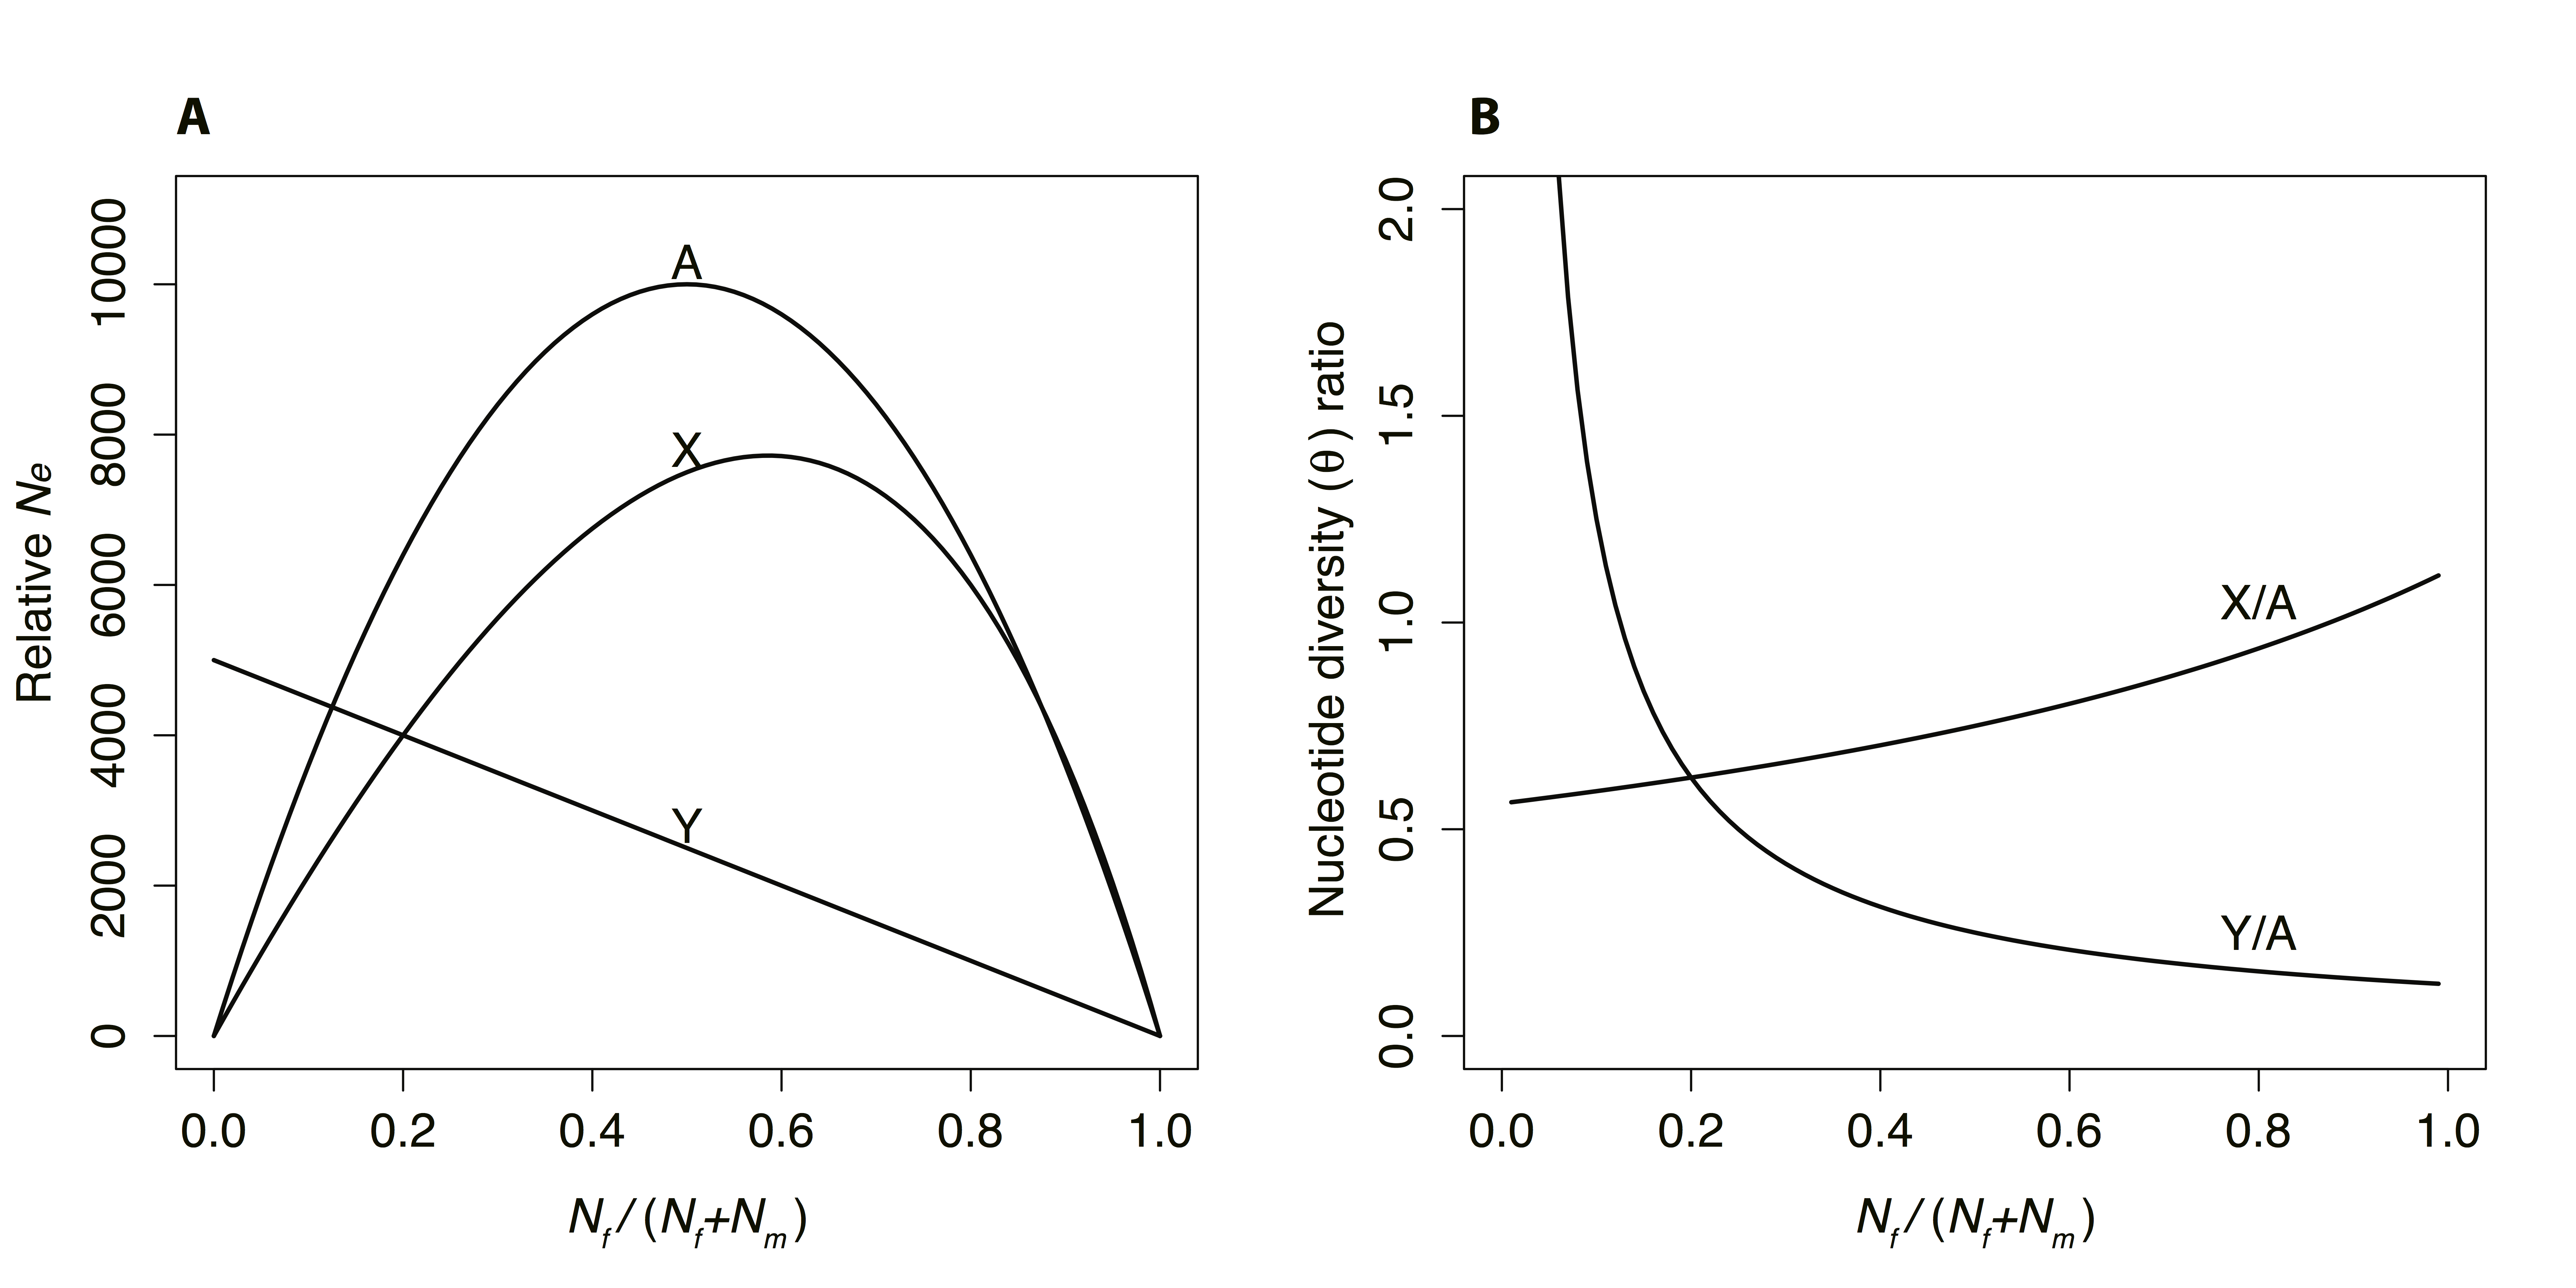
\includegraphics[width=\linewidth]{figure1.jpg}
\caption{\textbf{A}. Equilibrium effective population sizes, relative to $N$, for genes on autosomes, X chromosomes, and Y chromosomes as a function of the sex ratio. \textbf{B}. The corresponding X/A and Y/A ratios of nucleotide diversity predicted at equilibrium, assuming equal neutral mutation rates for sex-linked and autosomal genes.
}
\end{figure}

\subsection*{Simulations of purifying selection}
To study the effects of purifying selection on expected levels of Y-chromosome diversity, we conducted forward-time simulations of haploid Y chromosomes using the software SFSCODE \citep{hernandez2008flexible}. We first estimated the distribution of fitness effects of deleterious amino acid mutations from our polymorphism data for X-linked genes using the method of \citet*{keightley2007joint}, which fits a gamma distribution of negative selection coefficients to the observed frequency distribution of non-synonymous and synonymous polymorphisms. We then used this estimated gamma distribution to parameterize the simulations, initializing them with our estimated $\theta_{aut}$, adjusted to reflect the neutrally expected $N_{e_{Y}}$ for a sex ratio of $r = 0.6$. To match our sample size and the number of synonymous sites sampled from our data (see Supporting Information), the simulations sampled 6 haploid chromosomes, and the genome sequence contained 45,331 bp of linked neutral sequence from which we calculated silent site diversity, $\pi_{s}$. To examine the expected reduction in diversity as a function of the number of selected sites ($L$), we ran simulations over a range of values of $L$, up to a maximum of 5x$10^{6}$ (Figure 3). To obtain an estimate of $L$, we calculated the approximate likelihood of our observed data based on the proportion of simulations in which synonymous diversity, $\pi_{s}$, was less than 0.0001 from our empirical estimate (Figure 3B).

\section*{Results and Discussion}

\subsection*{Extensive loss of Y-chromosome diversity}
Our analysis of polymorphism levels across the genome in the dioecious plant \textit{R. hastatulus} reveals a widespread loss of neutral diversity from the Y chromosome. In particular, neutral diversity for Y-linked genes is on average \textasciitilde 2.1\% of the value for their homologues on the X chromosome. Taking 1/4 of the mean autosomal diversity as the equilibrium expectation for $\theta_{Y}$ under neutrality, this corresponds to a chromosome-wide reduction of 93\% relative to the standard neutral model \citep{wright1931evolution}. Note that by normalizing X and Y diversity estimates by autosomal diversity levels, our results indicate that the difference between X and Y homologues is not due to an elevation of diversity on the X chromosome, but a Y-specific reduction. Interestingly, our results also suggest an elevation of X-linked diversity ($X/A=0.85$) compared to the neutral prediction ($X/A=0.75$), though the confidence intervals on this estimate are wide, ranging from 0.74 to 0.95 (Figure 2). Given the empirically-estimated sex ratio of $r=0.6$ in \textit{R. hastatulus} \citep{pickup2013influence}, however, the X/A elevation we observed is not unexpected; the neutrally-predicted X/A ratio for a sex ratio of 0.6 is $\approx 0.8$ (Figure 2; Equation 4). Although our estimates of diversity have not been normalized by divergence, previous work has shown that the average synonymous substitution rate, between \textit{R. hastatulus} and the non-dioecious outgroup \textit{R. bucephalophorus} is comparable for sex-linked (0.2016) and autosomal genes (0.219), and we found no evidence for significant differences in substitution rate between Y and X chromosomes \citep{hough2014}. It is therefore unlikely that our results are caused by mutation rate differences between sex-linked and autosomal genes.

\begin{table}[htb]
\centering
\caption{Observed and neutrally-expected silent site diversity on sex chromosomes and autosomes in \textit{R. hastatulus}}
\begin{tabular}{ccccccccc}
\textbf{} & \multicolumn{2}{l}{\textbf{Observed}} & \multicolumn{3}{l}{\textbf{Expected}} \\

chr & $\theta$ & $/\theta_{aut}$ & $\theta$ & $/\theta_{aut}$  \\
\midrule
A & 0.0055 & 1 & N/A & 1 \\
X & 0.0047 & 0.85 & 0.0041 & 0.75 \\
Y & $\num{e-4}$ & 0.018 & 0.0014 & 0.25 \\
\addlinespace

\bottomrule
\end{tabular}
\end{table}

\subsection*{Female Biased Sex Ratios and Variance in Male Reproductive Success}
The occurrence of female-biased sex ratios in \textit{R. hastatulus} is expected to lower Y diversity through a reduction in male $N_{e}$ and thus a reduction in the $N_{e}$ of the Y chromosome. Male $N_{e}$ could be further reduced by high variance in male reproductive success, which is expected in annual wind-pollinated plants such as \textit{R. hastatulus} that commonly exhibit extensive phenotypic plasticity in plant size and flower production. Given that male plants in this species produce large amounts of pollen, and female flowers are uniovulate, there may indeed be strong competition among males to fertilize ovules. Such competition should cause a proportional increase in X-linked diversity to a level that is close to (or even higher than) levels of autosomal diversity \citep{caballero1995}, while simultaneously reducing Y-linked diversity. In common with most flowering plants, we do not have marker-based estimates of variance in male reproductive success in \textit{R. hastatulus}. We therefore tested whether an overall reduction in male $N_{e}$, arising either from high variance in male reproductive offspring number and/or a female biased population sex ratio, could explain our observed Y/A and X/A ratios, by comparing our data to neutral predictions across the full range of values for the $N_{e}$ sex ratio, $r$.

As shown in Figure 2, the expected reduction in Y/A as a function of $r$ is substantially higher than our observed Y/A diversity ratio. Indeed, the lower limit for the Y/A ratio in a neutral model is 1/8, such that even in the extreme case where $r=0.9$, the expectation for Y/A is $\approx 0.14$, which is substantially higher than our observed estimate ($Y/A= 0.018$) (Table 1; Figure 2). Moreover, such large reductions in $N_{e_{m}}$ would also predict levels of X/A diversity that are significantly larger than what we observed (Figure 2). Our results therefore indicate that, although reduced male $N_{e}$ arising from sex-biased demography is expected to contribute to reduced Y chromosome polymorphism, it is insufficient to explain the Y/A reduction we observed.

\begin{figure}[htbp]
\centering
\noindent
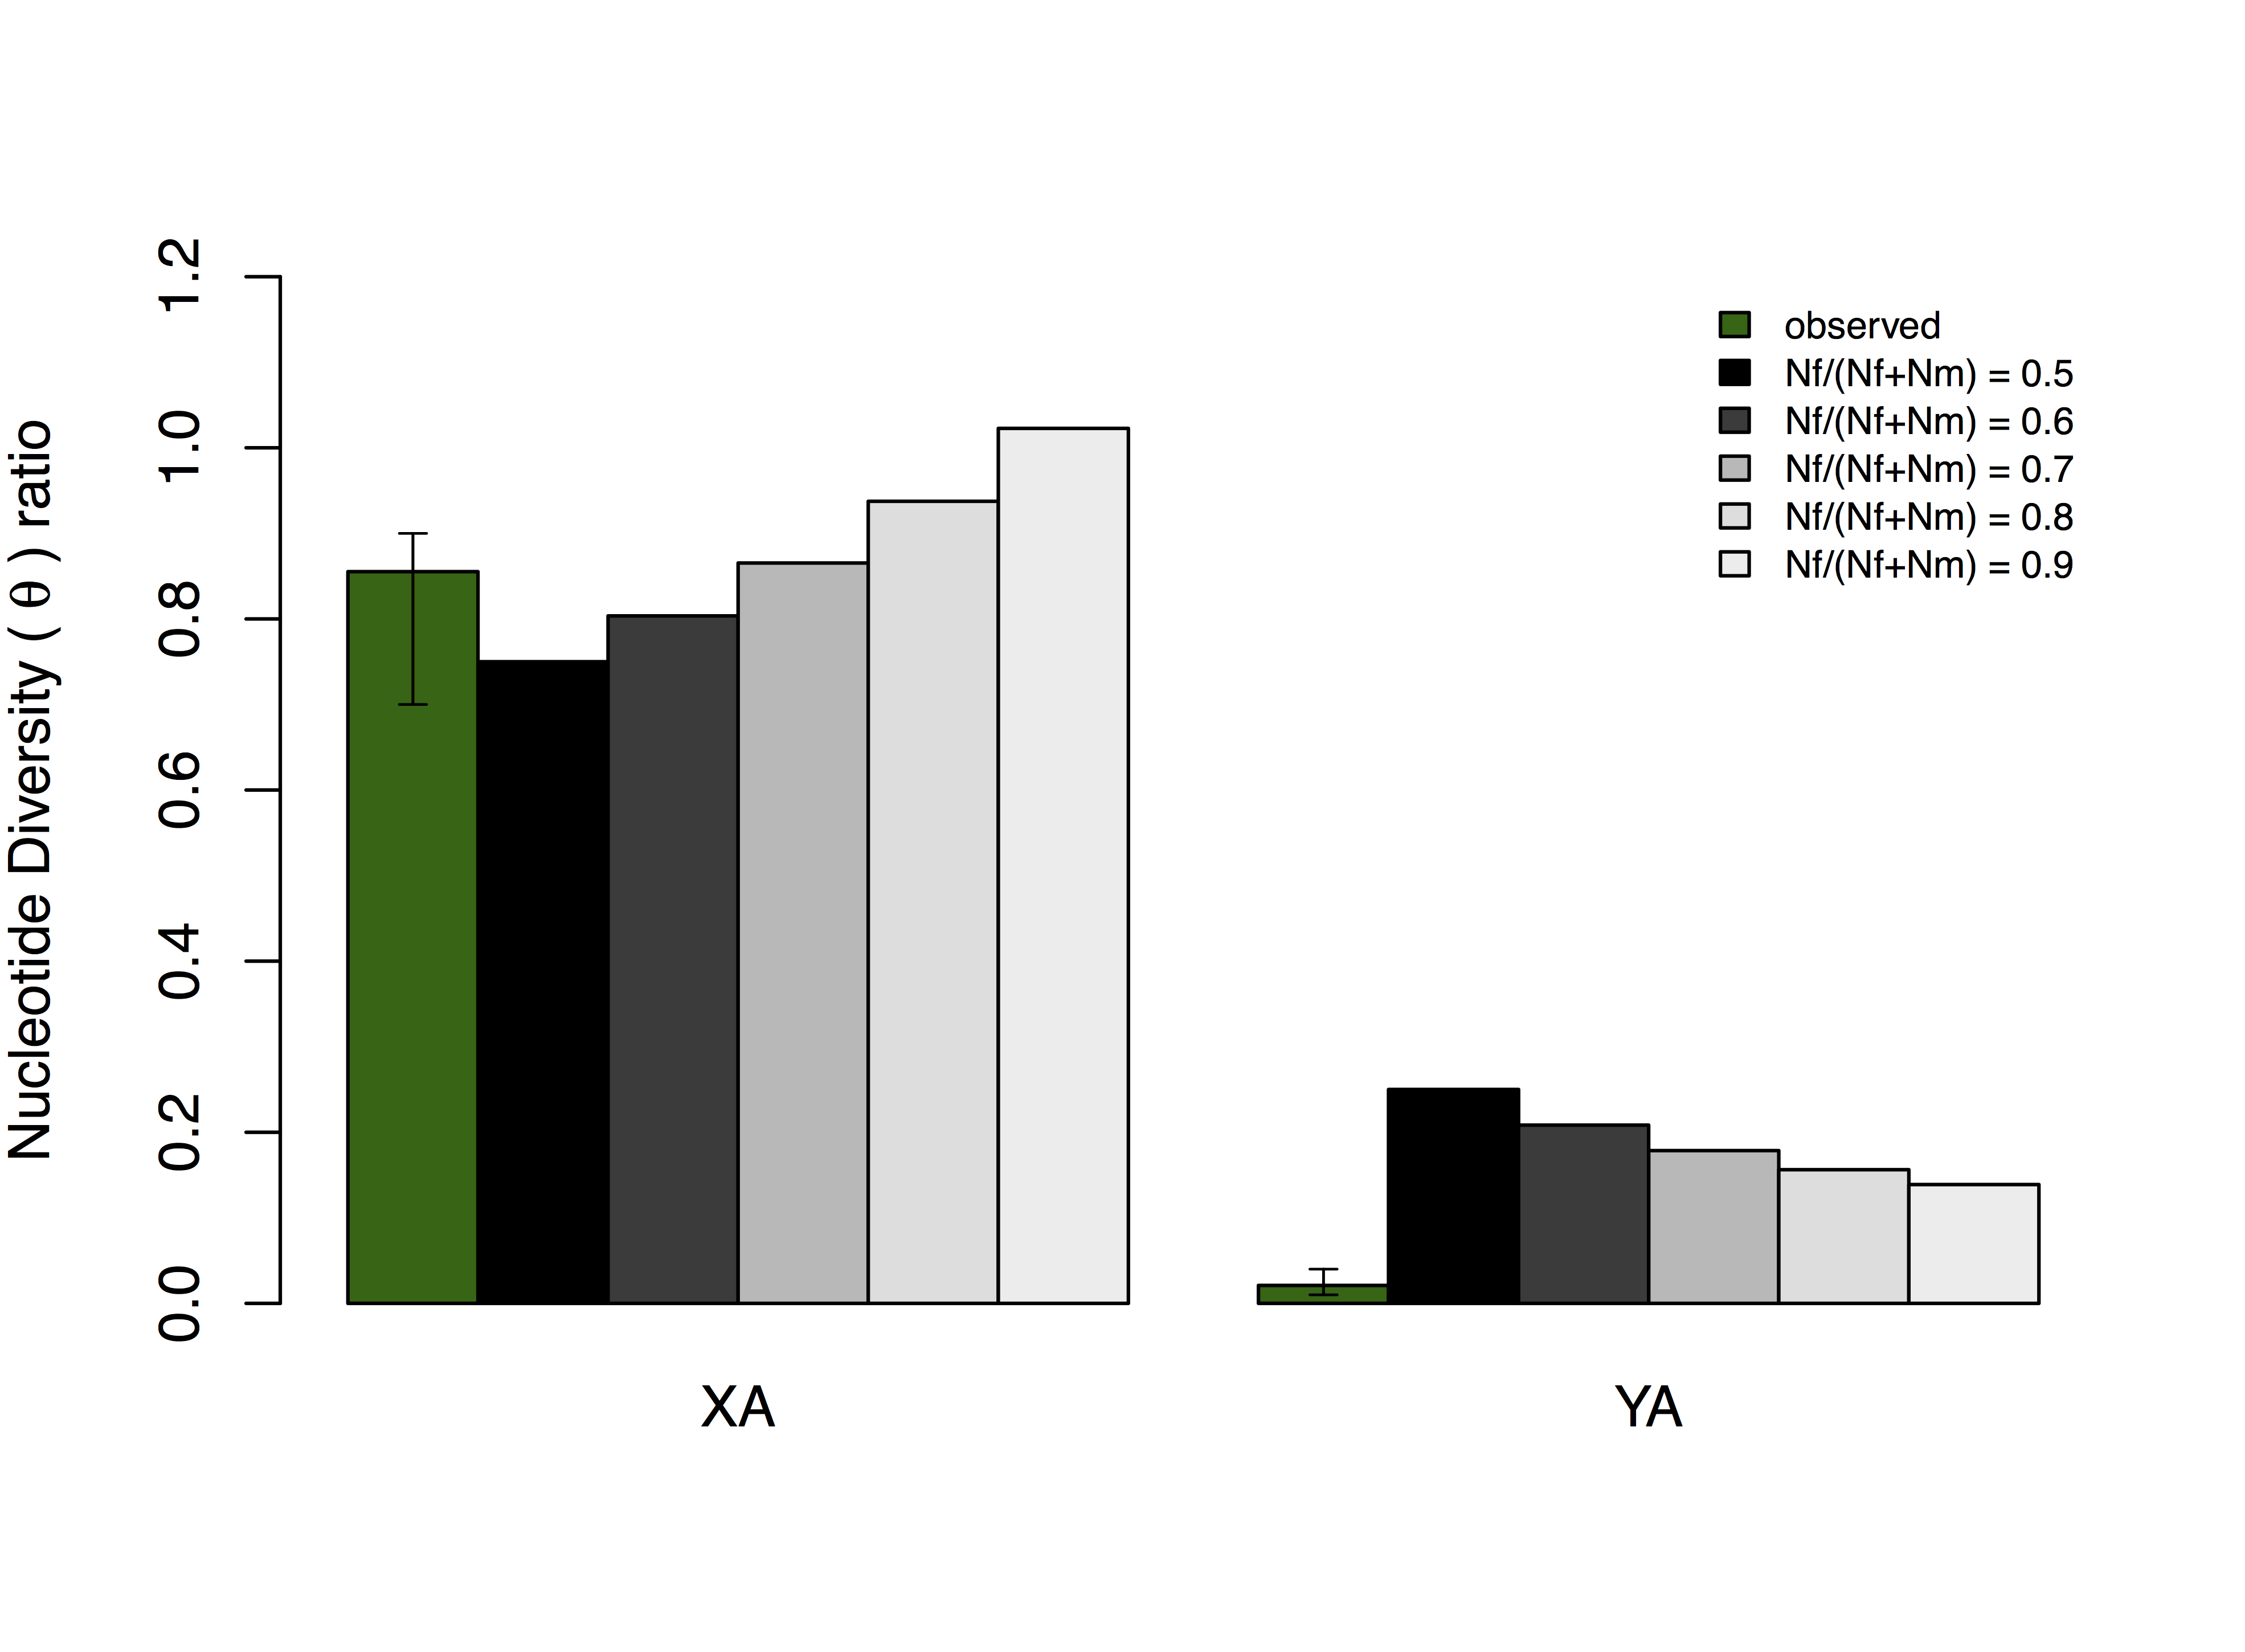
\includegraphics[width=\linewidth]{figure2.jpg}
\caption{Observed and predicted X/A and Y/A ratios of neutral diversity. Predictions are shown for increasing values of the effective population size sex ratio, $N_{e_{f}}/(N_{e_{m}} + N_{e_{f}})$. Observed estimates of X/A and Y/A were calculated as the average $\theta$ across genes, weighted by the number of synonymous sites per gene. Confidence intervals were calculated by bootstrapping (20000 replicates) using the BCa method \citep{efron1987better} implemented in the Boot package in R \citep{canty2012boot}, and using maximum likelihood for the Y-chromosome (see Methods).
}
\label{fig:ratios}
\end{figure}

\subsection*{Purifying selection}
Selection against strongly deleterious mutations is expected to be an important factor reducing genetic variability in regions with low recombination \citep{charlesworth1993effect, charlesworth1996background}. The effects of such “background selection” (BGS) have been well studied theoretically \citep{charlesworth1997effects, nordborg1996effect, kim2000joint} and the theory has been used to explain patterns of genetic diversity across genomes \citep{comeron2014background} and plays a central role in explanations for diversity loss on Y chromosomes in mammals \citep{Wilsonsayres2014} and \textit{Drosophila} \citep{mcallister1999, charlesworth1996CB}. Under background selection theory for a Y chromosome, the predicted loss of diversity is modeled as a reduction in the equilibrium $N_{e}$ such that $\pi \approx \pi_{0}=(\frac{Y}{A})4N_{e}f_{0}\mu$, where $f_{0}=e^{-\frac{U}{sh}}$, $U$ is the mutation rate to strongly deleterious variants on the Y, and $s$ and $h$ are selection and dominance coefficients \citep{hudson1995deleterious}. This yields the expected value of $\pi$ under the model: $E[\pi]=\pi_{0}e^{\frac{-U}{sh}}$, where $\pi_{0}$ is the expected diversity in the absence of BGS, $\pi_{0}=(\frac{Y}{A})4N_{e}\mu$, where Y/A is the expected ratio of the effective population size of the Y relative to autosomes. Here, assuming that the proportion of males is 0.4, and therefore that Y/A is 0.21 of the total $N_{e}$ estimated from autosomes as a result of the female biased sex ratio in \textit{R. hastatulus} \citep{pickup2013influence}, and using $s$=0.003 as estimated from the distribution of fitness effects of deleterious mutations, the corresponding expected diversity on the Y chromosome under BGS is $E[\pi]$= 1.5x$10^{-5}$ for a haploid Y chromosome mutation rate of 7x$10^{-9}$ per nucleotide per generation and 1 MB of selected sites. Although there is considerable uncertainty in these parameters, the calculation yields an expected value of diversity that is 70\% lower that what we observed (Table 1; Figure 2; Figure 4).

\begin{figure}[t!]
\centering
\noindent
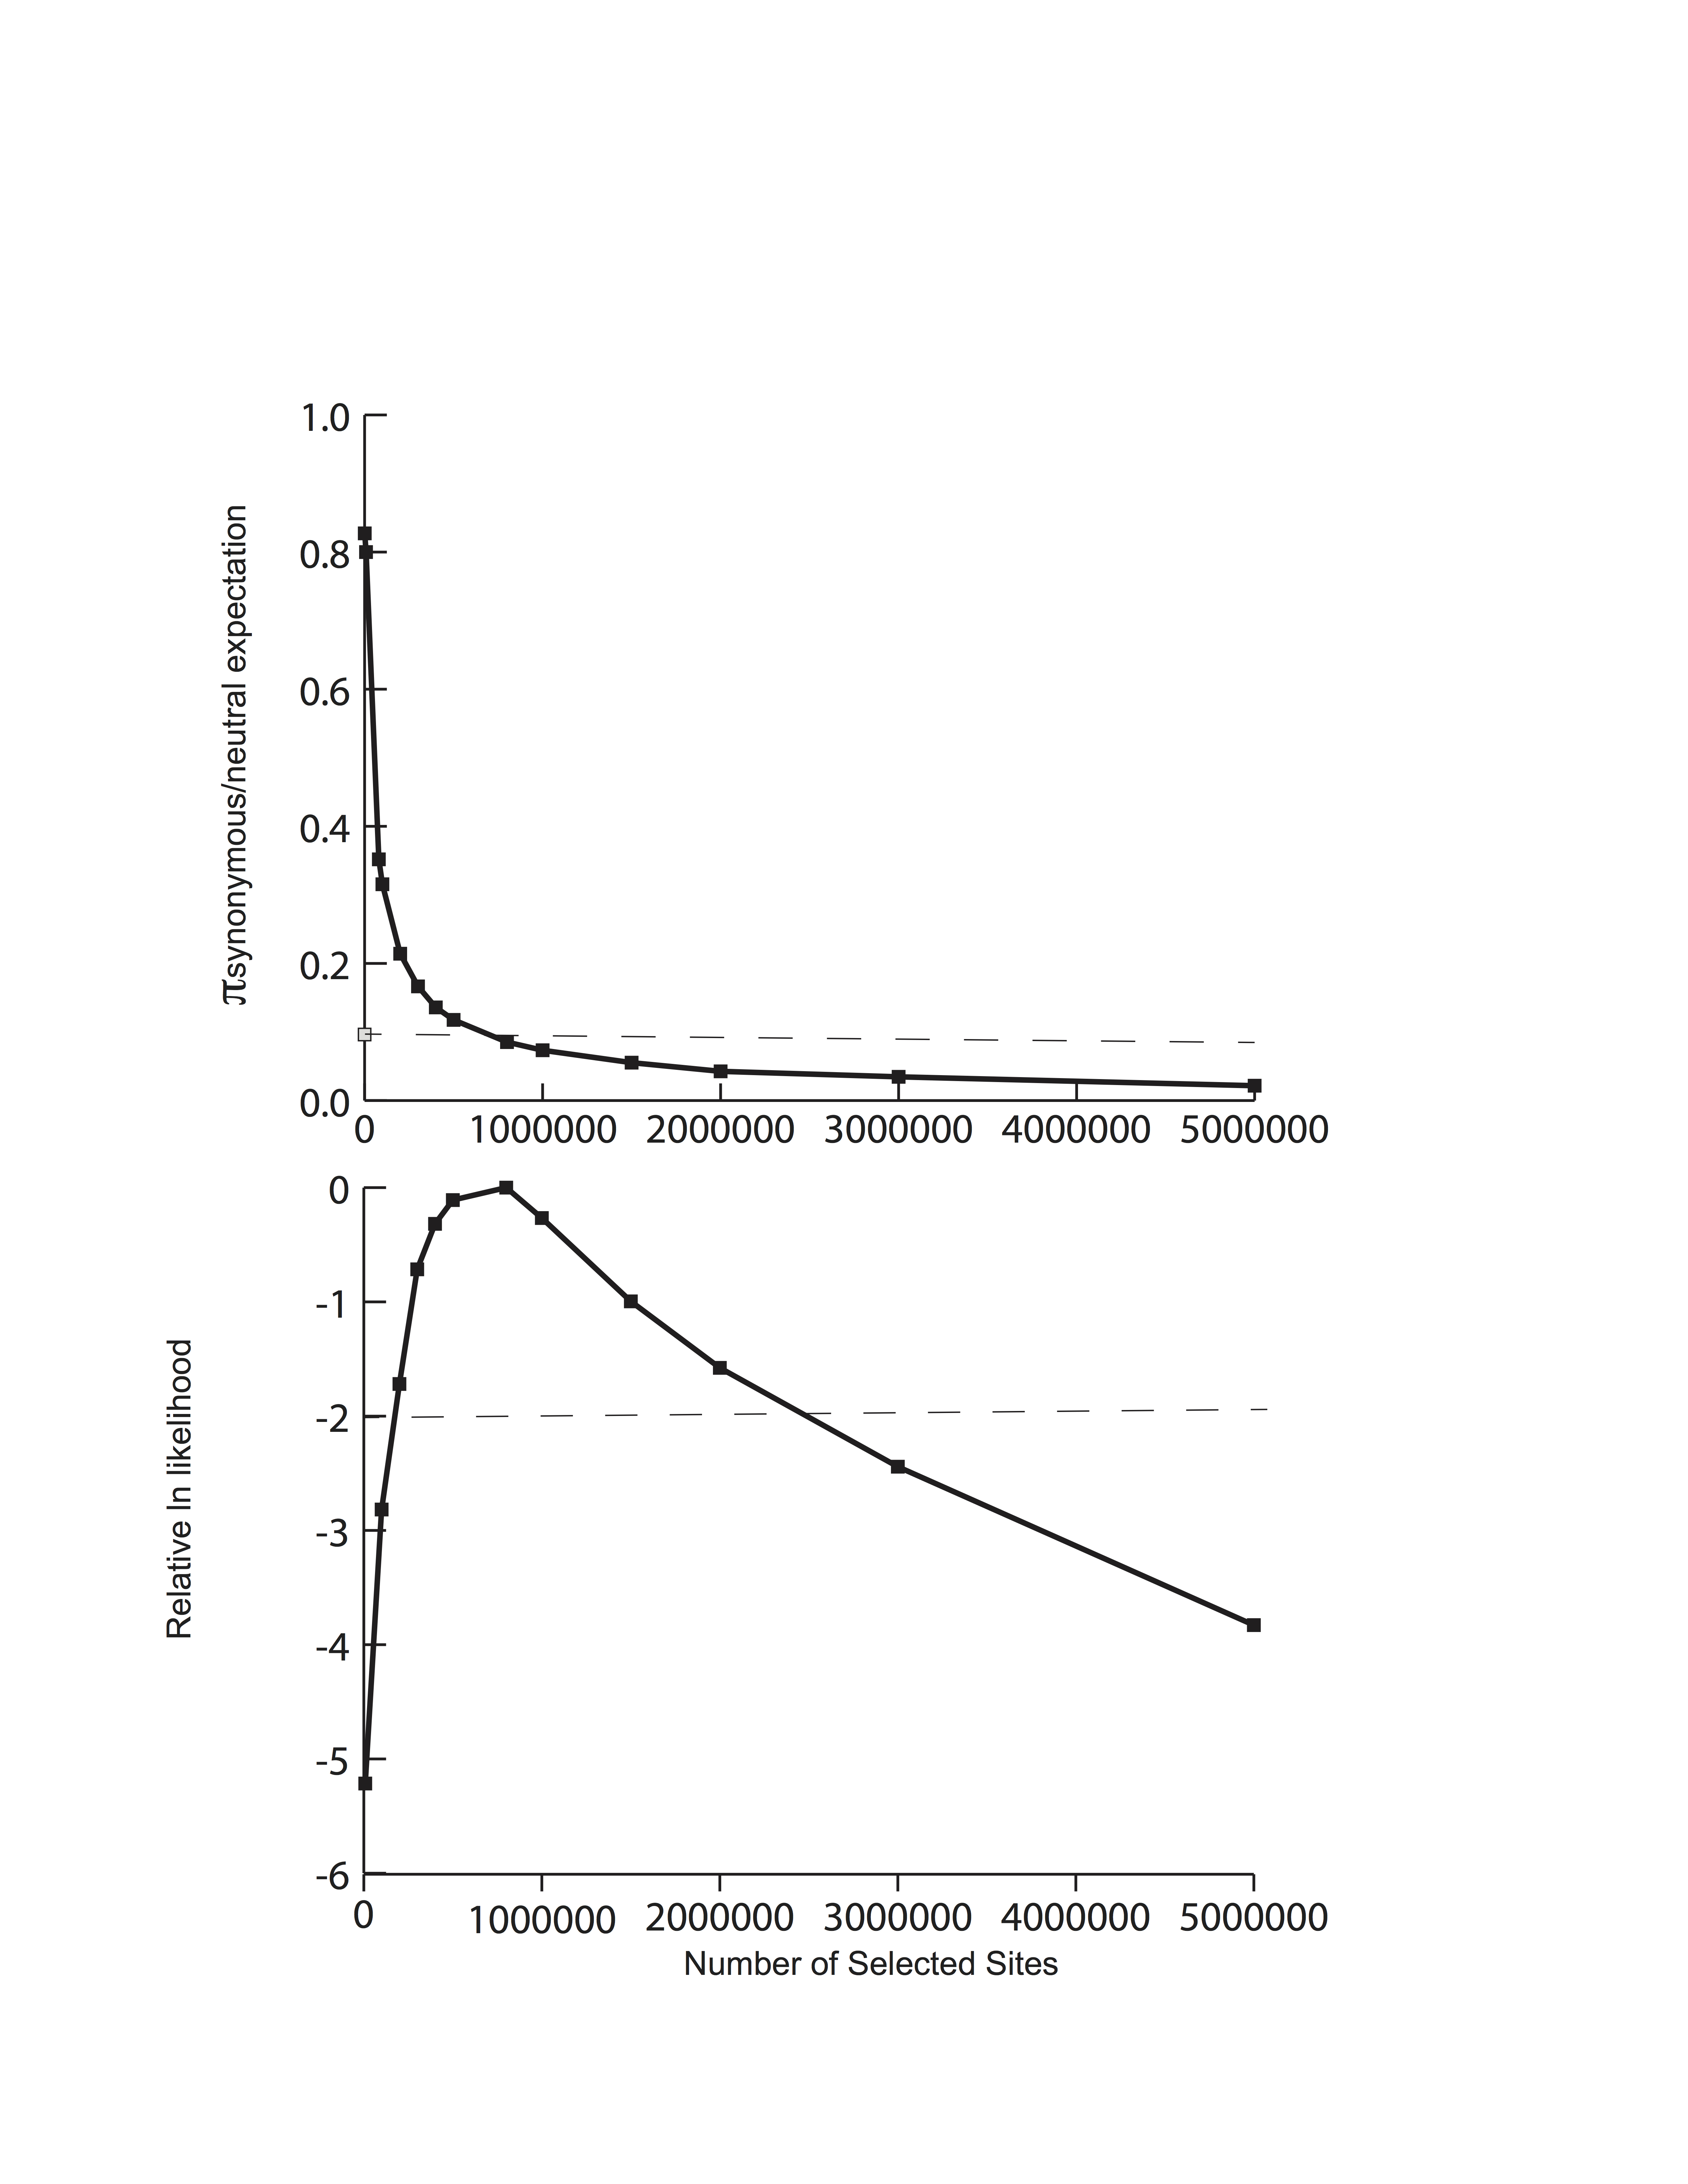
\includegraphics[width=\linewidth]{figure3.jpg}
\caption{Results from forward simulations of purifying selection. Top: estimated silent site diversity $\pi$ relative to neutrality ($\pi_{0}$) as a function of the number of selected sites. The dashed line corresponds to our estimate of diversity on the Y chromosome ($\theta_{Y}$). Bottom: the relative likelihood curve for the number of selected sites, with the dashed line reflecting the approximate 95\% credibility interval.
}
\label{fig:selectedsites}
\end{figure}

Importantly, BGS assumes independence among sites, and the theory breaks down when many linked sites are subject to selection at the same time. This isbecause high linkage disequilibrium causes the behavior of selected alleles interfere with the action of selection at linked sites \citep{good2014genetic,KaiserCharlesworth}. As there are no analytical formulae for predicting the outcome of selection on many linked alleles experiencing selection and drift, however, simulations are fundamental to understanding such selective interference in realistic situations. We therefore conducted forward simulations of purifying selection using our estimated parameters for the distribution of fitness effects of deleterious mutations, and tested whether interference selection could result in a level of Y diversity at neutral sites similar to the level we observed.  Our maximum likelihood estimates of the number of selected sites, $L$, from our simulations, suggest that the number of sites subject to selection required to explain the diversity loss from the \textit{R. hastatulus} Y chromosome is ($\approx 800 kb$) and may be as large as 2.5 MB (Figure 3). Thus, these results are consistent with the hypothesis that the early stages of Y degeneration are characterized by the persistence of a large number of sites subject to purifying selection.

While clearly approximate, we can ask how these estimates compare to how many selected sites we might expect to be present on the Y chromosome. Our previous estimates based on cytological measurements suggested that there may be roughly 5,600 genes on the X chromosome of the XY race \citep{hough2014}. We also estimated that approximately 28 percent of genes had degenerated, leaving us with an estimated 1568 genes remaining on the Y chromosome. Using the average number of codons in genes of \textit{Arabidopsis thaliana} (426) \citep{wortman2003annotation}, and assuming 2/3 of codons are under selection, this would imply 1.3 MB of selected sites, which is well within the range of our uncertainty (Figure 3). Thus, although our estimates are broad, these results are consistent with the retention of a large proportion of sites subject to purifying selection on the Y chromosome, as expected in the early stages of degeneration.

\begin{figure}[t!]
\centering
\noindent
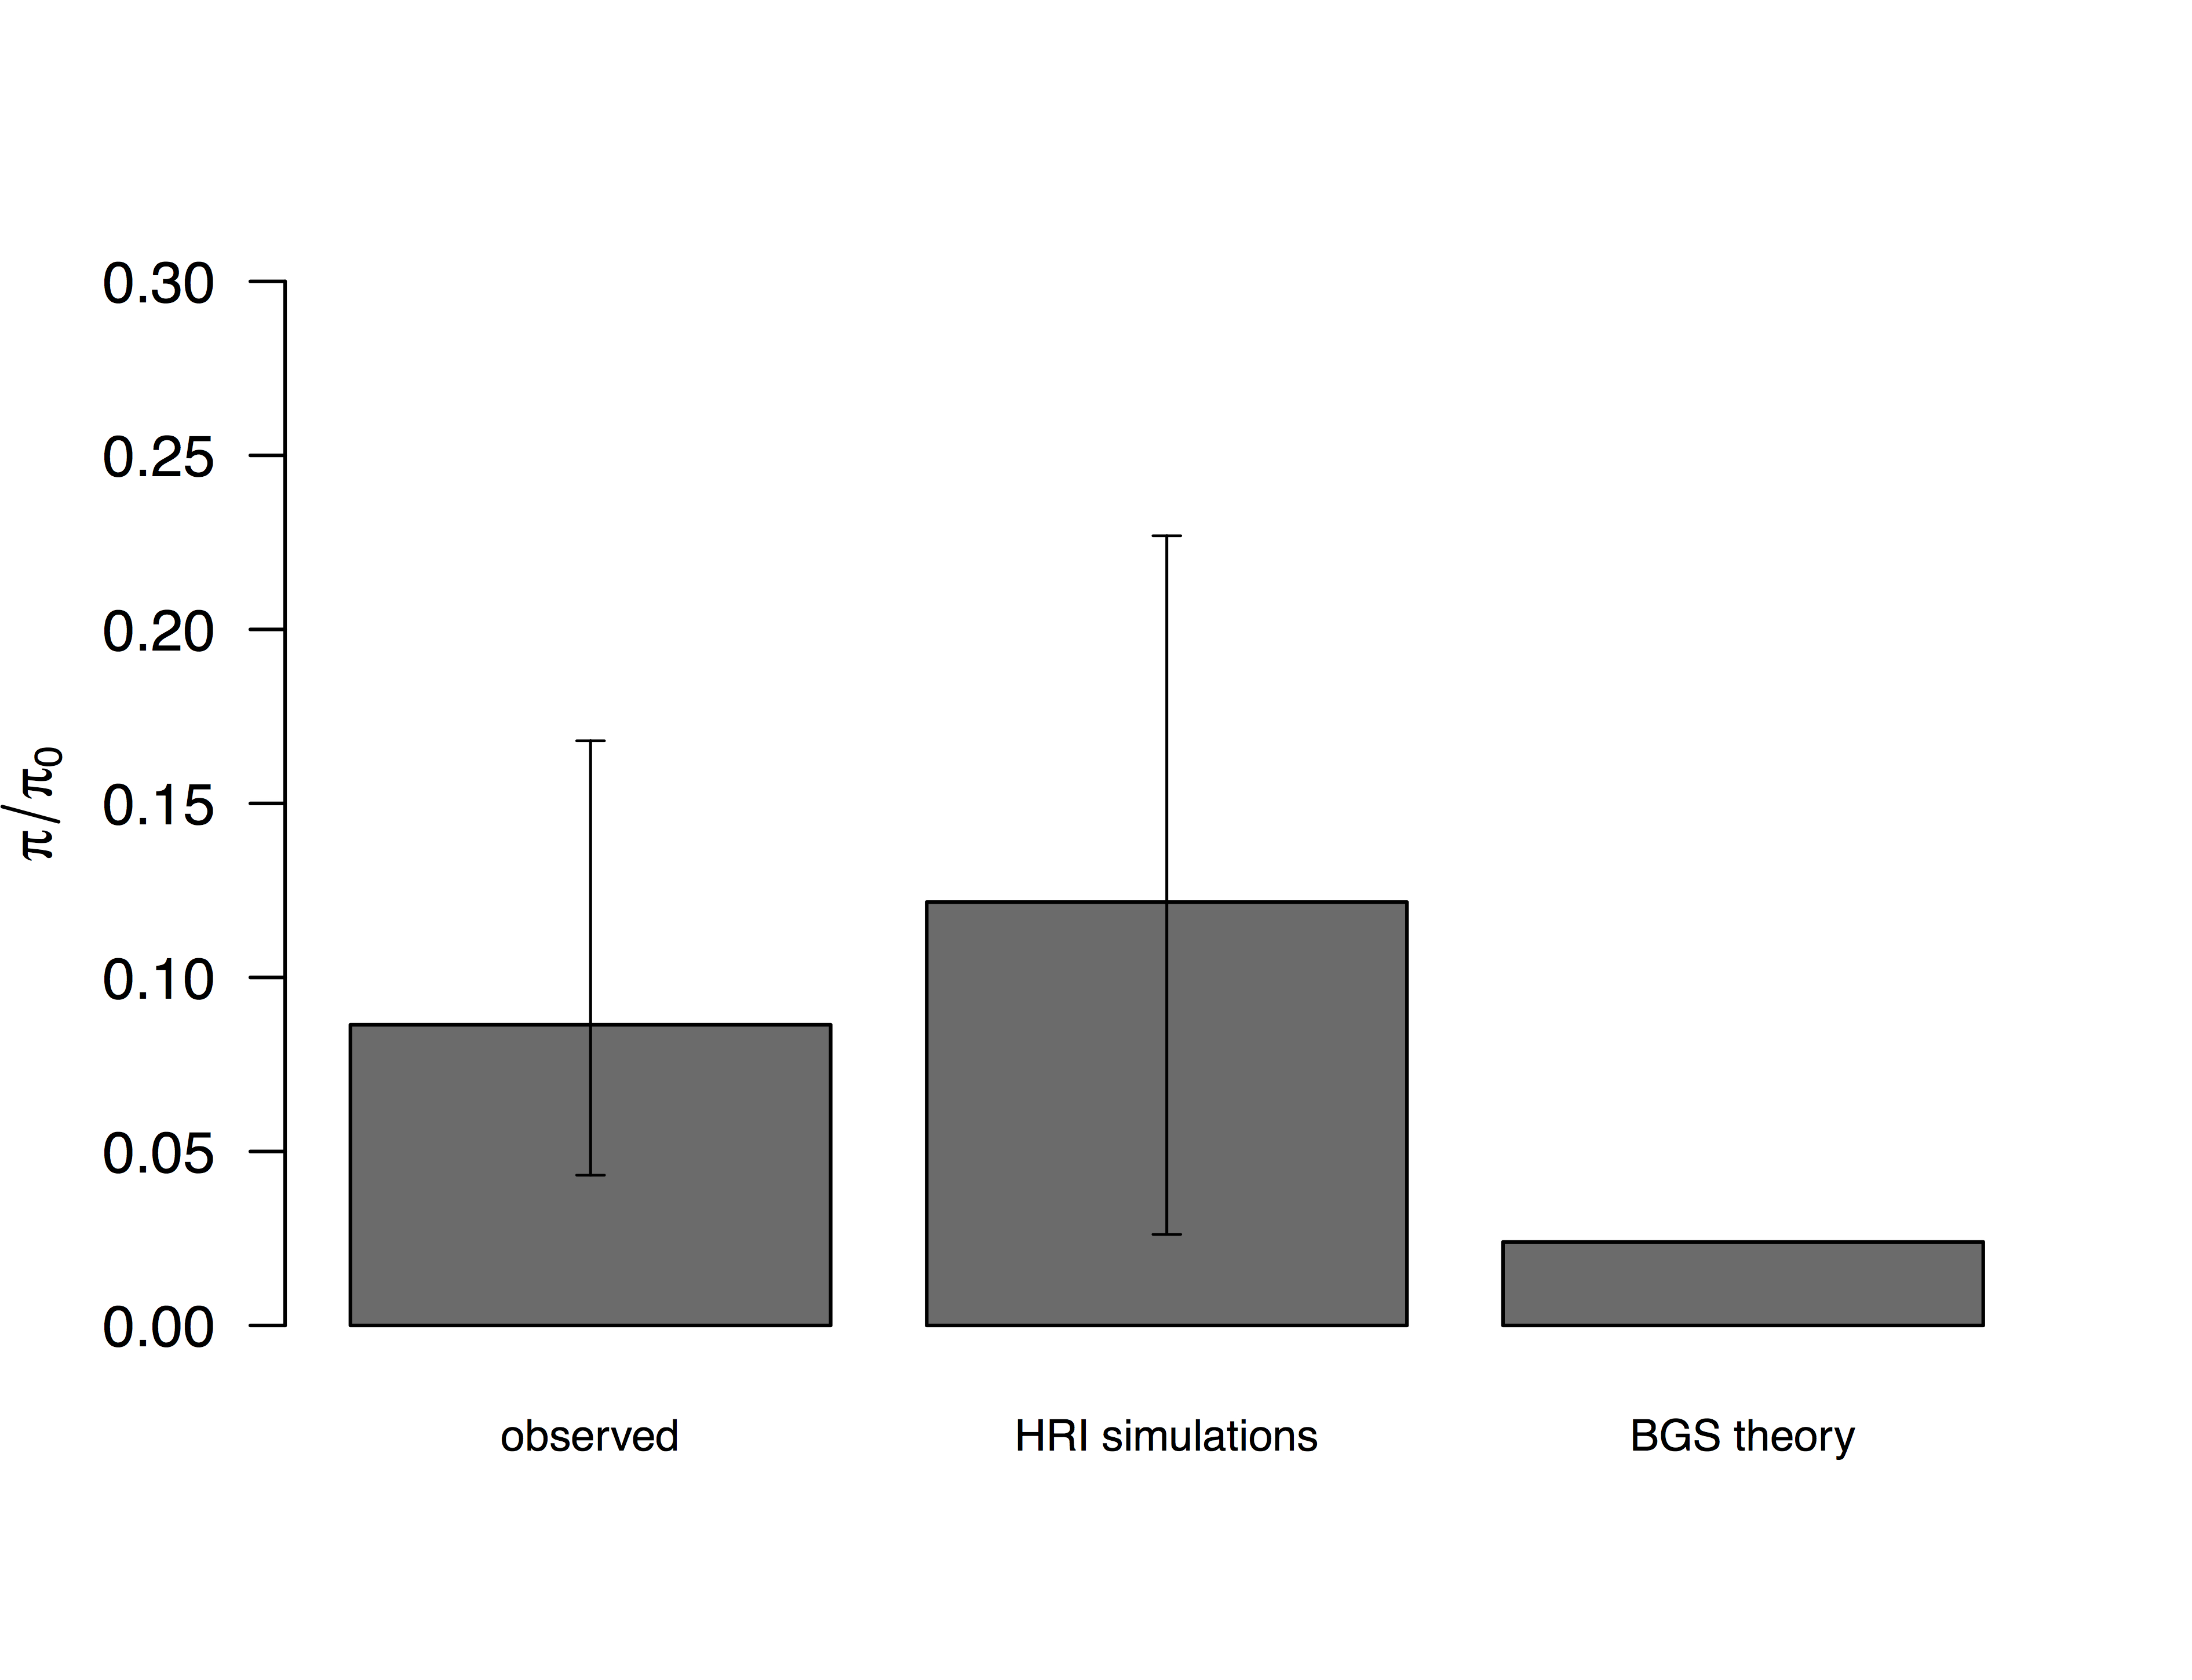
\includegraphics[width=\linewidth]{figure4.jpg}
\caption{Estimated levels of Y-linked nucleotide diversity compared to estimates obtained from simulations of purifying selection among linked selected sites (HRI simulations) and analytical predictions from background selection theory. Silent site diversity is reported relative to the neutral expectation ($\pi_{0}$), where $\pi_{0}=(\frac{Y}{A})4N_{e}\mu$, and Y/A is the expected ratio of the effective population size of the Y relative to autosomes for a sex ratio of $r=0.6$, as estimated in \textit{R. hastatulus} populations. The credibility interval for our observed Y diversity was obtained by maximum likelihood (see methods), and error bars for HRI simulations correspond to 1.5x the interquartile range for $\pi_{s}$ estimates, approximately equal to the 95\% confidence interval for the median \citep{chambers1983graphical}.
}
\label{fig:ydiversity}
\end{figure}

Although our analyses of purifying selection models are consistent with our observed reduction in Y-linked diversity, it is also possible that selective sweeps have contributed. We have not formally excluded this possibility. However, if patterns of molecular evolution on the Y are driven primarily by interference selection, as our results suggest, then a further implication is that beneficial mutations should suffer a reduction in their probability of fixation, limiting the scope for sweeps to drive down diversity. Nonetheless, there is abundant evidence that “soft sweeps” are important determinants of patterns of nucleotide diversity \citep{messer2013population}, and it is possible that they have contributed to the extremely low levels of Y-linked variability that we observed.

\section*{Conclusions}
The non-recombining region of a Y chromosome produces evolutionary dynamics that are similar to a haploid asexual population, with the lack of recombination resulting in build up of genetic associations among selected sites, a loss in the efficiency of selection, and an increase in population fitness variance \citep{fisher1930genetical, muller1964relation, hill1966HReffect, mcvean2000,KaiserCharlesworth,good2014genetic}. Our study of neutral diversity levels on the relatively young \textit{R. hastatulus} sex chromosomes provides clear evidence for an extensive loss of neutral diversity on the Y chromosome. Whereas neutral models of sex-biased demography were unable to explain the magnitude of diversity loss, forward population genetic simulations suggest that the extensive loss of diversity is most likely due to purifying selection. However, while standard background selection theory over-predicted the loss of diversity on the Y chromosome by $\approx$ 70\%, simulations of purifying selection acting over a large number of linked selected sites resulted in a level of Y-diversity that was similar to what we observed. These results are consistent with theory on interference selection, and suggest that the effects of interference is likely an important force in the evolution of young Y chromosomes. Moreover, our results imply that when a large number of linked sites are subject to purifying selection, Y-chromosome degeneration in the early stages may largely be driven by the effects of interference rather primarily by widespread silencing of Y-linked genes and their subsequent degeneration through neutral drift.

\section*{Acknowledgments}
We thank Felix Baudry for providing genomic coverage data for quality filtering. This research was funded by Discovery grants to SCHB and SIW from the Natural Sciences and Engineering Research Council of Canada, and by an OGS scholarship to JH.

\bibliography{bibliography}
\end{document}